\doublespacing % Do not change - required

\chapter{Implementation}
\label{ch4}

%%%%%%%%%%%%%%%%%%%%%%%%%%%%%%%%%%%%%%%
% IMPORTANT
\begin{spacing}{1} %THESE FOUR
\minitoc % LINES MUST APPEAR IN
\end{spacing} % EVERY
\thesisspacing % CHAPTER
% COPY THEM IN ANY NEW CHAPTER
%%%%%%%%%%%%%%%%%%%%%%%%%%%%%%%%%%%%%%%
\section{Discuss the practical realization of the proposed method}
In this section, practical implementation of smart energy monitoring and control system using Modbus protocol and Programmable Logic Controller (PLC) will be discussed. The system was designed to perform real-time data collection, analysis and control functions via a simulation program in order to increase energy efficiency and optimize energy consumption. The aim of the project is to monitor, optimize energy use in industrial facilities and reduce environmental impacts.

The basis of the system is to transfer energy data received from sensors to a PLC via Modbus protocol and process this data to optimize energy consumption. Here, a production system was implemented in Factory IO environment and then the PLC code suitable for this system was tried to be written via PLC software. PLC collects and processes data from sensors and will undertake the task of activating the control algorithm to improve the energy consumption of the system. It was decided to implement PID (Proportional-Integral-Derivative) as the control algorithm considered in this project. Both the simple and effective structure of the controller and its compatibility with PLC were effective in this decision. The purpose of using controllers is to turn devices on and off or adjust their speeds as necessary in order to minimize energy consumption and maximize system efficiency.
a
The simulation of the system in a virtual environment was performed with Factory IO software. This software has the ability to model and simulate industrial automation processes in a 3D environment and can be integrated with PLC and other automation systems. The simulation allowed the system to be tested in the real world and allowed the system to be evaluated without implementing a real application, considering the time and cost calculations.

The PLC used in the project process is the Siemens S7-1200 model. This model has high compatibility with the Modbus protocol and is widely used in industrial automation systems thanks to its fast processing capacity and expandable structure. In this project, a virtual PLC provided by Siemens, known as the PLCSIM application, was used instead of a real PLC. In the study, v18 versions were used in both programs. PLC Siemens S7-1200 was preferred due to the convenience of operating the PID control block and its compatibility with other programs.

The structure of the system components will be detailed below:

\textbf{Sensors:}: 

In order to control energy consumption, energy-related information such as speed, position, current of energy consuming system components must be known by the user. In this system, there are a number of power consuming components in the simulation environment. These are components such as conveyor systems that enable the movement of products in the system, robot arm that changes the position and state of the product. The robot arm transmits data to the PLC via the enerModbus protocol and fulfills the energy monitoring function by providing instant data for each energy parameter. 

\begin{figure}[H]
    \centering
    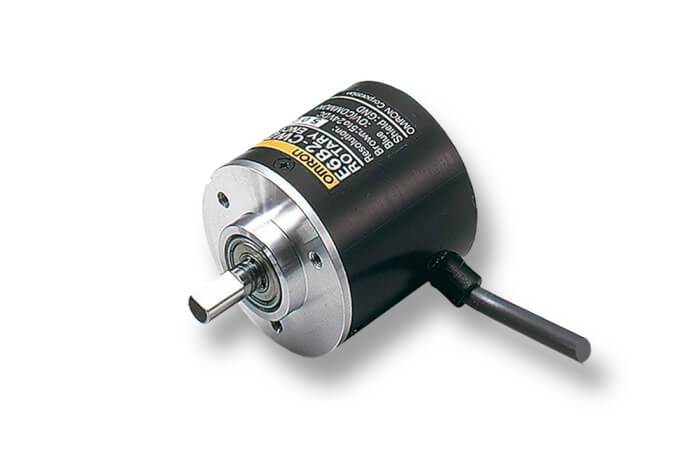
\includegraphics[width=0.8\columnwidth]{encoder.jpg}
    \caption[e6b2-c Encoder]{e6b2-c Encoder}
    \label{fig-magnitude}
\end{figure}%

\textbf{PLC (Programmable Logic Controller)}: 

A control device used in industrial automation systems. Siemens S7-1200 PLC is a widely used model in such systems and is known for its high performance. PLC usually communicates with sensors, actuators and other devices to control various processes. Such controllers analyze incoming data, apply certain logical operations and send output commands to make the system work more efficiently. One of the most important features of Siemens S7-1200 PLC is its compatibility with industrial protocols such as Modbus TCP/IP and Modbus RTU. These protocols allow PLC to exchange data with different devices and systems, thus ensuring seamless integration between devices.

\begin{figure}[H]
    \centering
    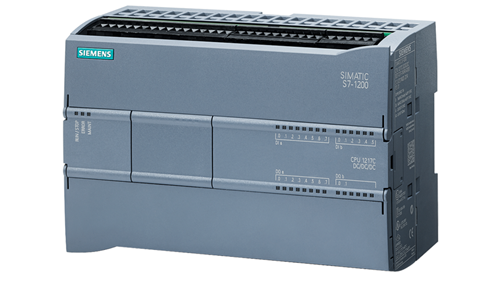
\includegraphics[width=0.8\columnwidth]{imgs/s7-1200.png}
    \caption[S7-1200 PLC]{S7-1200 PLC}
    \label{fig-magnitude}
\end{figure}%

\textbf{Communication Protocols:} 

Modbus is a communication protocol widely used in industrial automation systems. Designed to provide data transmission and communication between devices, this protocol allows data received from sensors to be processed securely and quickly, especially in PLC (Programmable Logic Controller) systems. There are different versions of Modbus; the most common of these are Modbus RTU (Remote Terminal Unit) and Modbus TCP/IP (Transmission Control Protocol/Internet Protocol).

In the Modbus RTU module, data is transmitted in digital format and communication is generally established over serial connections (such as RS-232, RS-485). This version is preferred in low-cost and simple systems because it has sufficient features in terms of speed and security. The RTU format provides error control and data verification mechanisms in each data frame, ensuring the security of data transmission.

Modbus TCP/IP, on the other hand, uses an Ethernet-based system and transmits data over the network using internet protocols. This version is preferred in larger systems, when a large number of devices need to be connected to each other. Modbus TCP/IP optimizes data communication in industrial automation systems by offering higher speeds and more device support.

\textbf{Control Algorithms}  

PID controller is a control system widely used in industrial automation and engineering applications, and includes Proportional (P), Integral (I), and Derivative (D) components. These components are combined to minimize the error between the target value and the current value of a system. PID controller is generally used to control temperature, speed, pressure, and other physical quantities. The basic components of PID control are explained below:

Proportional (P): The proportional component produces a control signal proportional to the error. The error is the difference between the target value and the actual value. This term determines the response speed of the system. A high Kp (proportional gain) value allows faster response to the error, but an excessively large Kp value may cause the system to be unstable.

Integral (I): The integral component takes into account the accumulation of the error over time. This term increases the error reset ability of the system and is used to eliminate static errors. However, a very large Ki (integral gain) value may cause the system to oscillate.

Derivative (D): The Derivative component takes into account the rate of change of the error. This term allows the system to reach equilibrium more smoothly and quickly. The value of Kd (derivative gain) helps to reduce the oscillations of the system, but a very high value of Kd can create excessive sensitivity in the system

\medskip

\section{Provide details on system architecture, hardware/software implementation}
\subsection{Software Programs}

Here, the software programs used in the project will be introduced first and their functions will be mentioned in the project. Then, hardware and software applications related to the system will be explained.

Many different software programs were used together in the system. What they are and their roles in the project are as follows:

\begin{itemize}
    \item \textbf{Matlab:} MATLAB (Matrix Laboratory), is a powerful software environment used for mathematical computations, data analysis, engineering and scientific research. Developed by MathWorks in the late 1980s, this software is widely used in many areas such as numerical computations, data analysis, graphics, simulations and algorithm development.

MATLAB is a matrix-based software environment, which is one of its most powerful features. While it focuses primarily on processing numerical data, it offers advanced mathematical functions, graphical tools, and a user-friendly programming language. MATLAB is often used in areas such as engineering calculations, control systems, signal processing, image processing, machine learning, and artificial intelligence.

MATLAB has a large number of built-in functions and toolboxes. Users can develop customized solutions in different application areas. For example, Simulink is a tool used with MATLAB for simulations of dynamic systems. It also allows users to visualize.

This project includes electric motors that drive the movement of robot arms and conveyors. Matlab was used to create models of these DC motors in the system and to relate the relationships of various physical quantities to each other and to energy.
\end{itemize}

\begin{itemize}
    \item \textbf{Tia Portal ve PLCSim:} TIA Portal (Totally Integrated Automation Portal) is a software platform developed by Siemens and provides integrated management of all components of industrial automation systems. This software allows users to program and monitor various devices such as PLC (Programmable Logic Controller), HMI (Human Machine Interface), motors, sensors. TIA Portal simplifies the software development, monitoring and maintenance processes of automation systems. Users can manage automation projects in an integrated manner through a single platform and accelerate the design process. This software is designed specifically for Siemens S7 PLCs and the Simatic product family and is widely used in production lines and industrial facilities.

    PLCSim is a simulation software that works integrated with Siemens' TIA Portal. This software allows PLC programs to be run in a virtual environment. PLCSim helps engineers verify their software by simulating software development and testing processes before using real hardware. This software is extremely useful in training and development processes, detecting programming errors and foreseeing the operation of automation systems.

    In this project, TIA Portal software was used to control the industrial production line simulation created in the Factory IO environment via a virtual PLC. This program written via the TIA portal was connected with the PLCSim selection from the drivers section in the Factory IO section and the inputs and outputs were matched and controlled. The program belonging to the project can be seen in detail in Appendix-1.
\end{itemize}

\begin{itemize}
    \item \textbf{Factory IO:} Factory IO is a simulation program used to model, test, and train industrial automation applications. Factory IO is used to perform simulations of PLC (Programmable Logic Controller) based systems, thus ensuring that industrial automation systems are designed and tested correctly.

    Factory IO includes devices such as a virtual production line, conveyor belts, robots, sensors, and actuators. These devices can be controlled with industrial protocols such as Modbus TCP/IP, allowing the user to test PLC programs without requiring real hardware. One of the biggest advantages of Factory IO is that it is compatible with industrial programming software such as TIA Portal or RSLogix 5000. This compatibility facilitates system integration and allows engineers to develop their software faster and more efficiently.

    Factory IO is used not only for simulation and training purposes, but also for the development of robotic systems, system design, and pre-application testing in the field. Users can simulate various industrial scenarios and applications in the software and increase the efficiency of the system by performing tests on these simulations. In addition, the software provides the necessary tools for users to test PLC programs, perform system verification, and perform performance analysis.
    
    As will be explained in detail in the following sections of this project, a simulation environment was created in the Factory IO environment where two parts will be combined. Then, the program was connected to the virtual PLC via PLCSim and the process was controlled from there.
\end{itemize}

\subsection{Created Project Environment}
This project includes a simulation program that involves producing two different parts that have key-lock compatibility with each other and then integrating them with a robot arm. As mentioned before, Factory IO, which produces a prototype of the real industrial world, was used as the simulation program. Figure 4.3 below shows the empty world of the Factory IO program.

\begin{figure}[H]
    \centering
    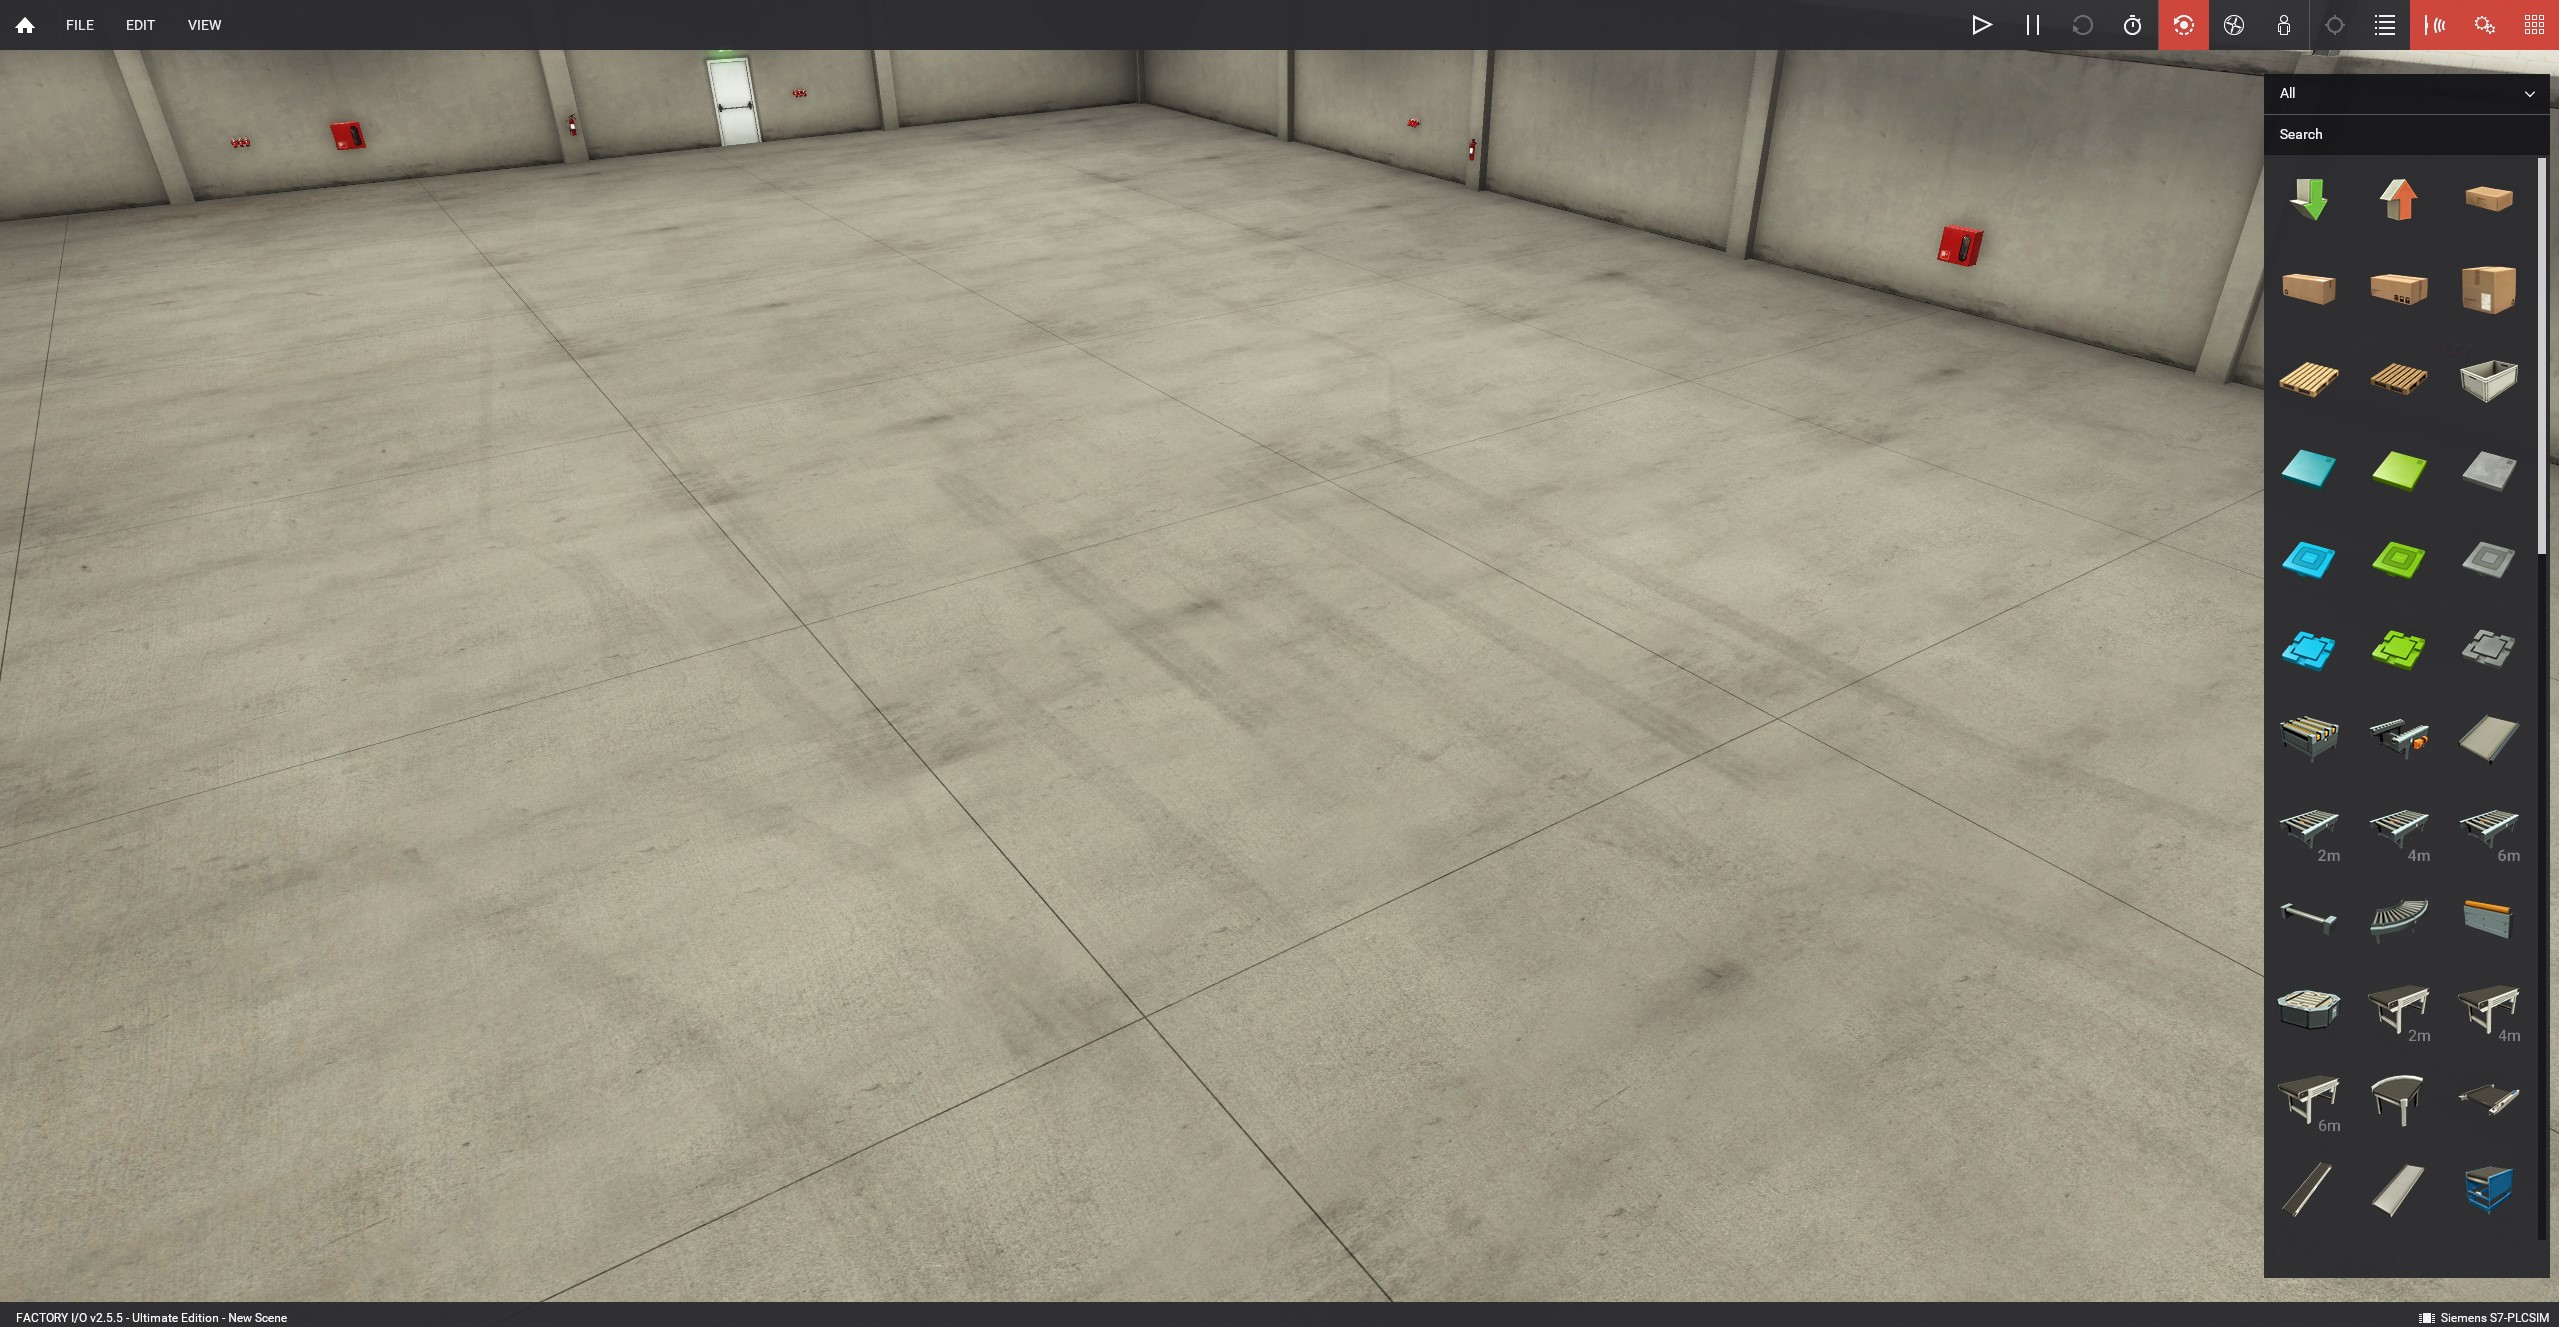
\includegraphics[width=0.5\columnwidth]{FactoryIO_baslangic_ortami.jpg}
    \caption[Factory IO starting environment]{Factory IO starting environment}
    \label{fig-magnitude}
\end{figure}%

As explained above, the project includes a simulation program that combines two parts. Below is a detailed examination of the system and an explanation of its working logic.

Below is the front view of the simulation system created in Figure 4.4.
\begin{figure}[H]
    \centering
    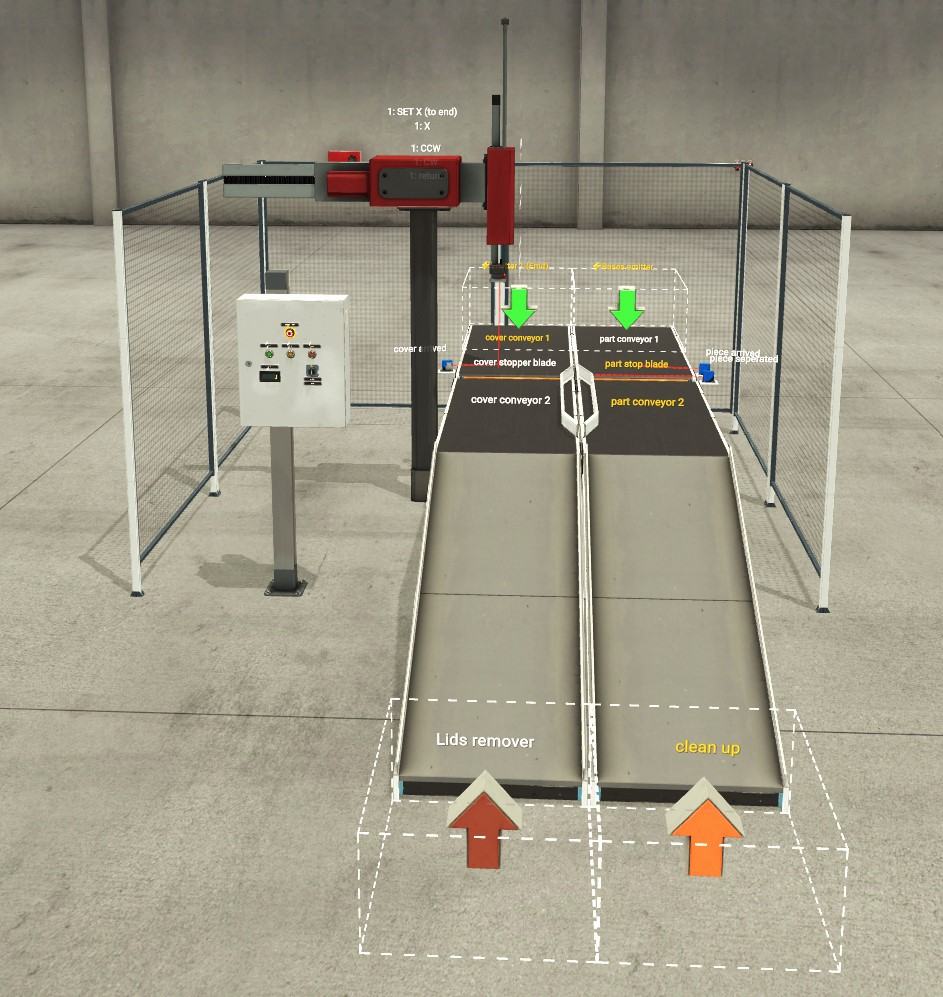
\includegraphics[width=0.5\columnwidth]{imgs/io/3.jpg}
    \caption[Front view of the created system]{Front view of the created system}
    \label{fig-magnitude}
\end{figure}%

The right view of the simulation system is shown in Figure 4.5.
\begin{figure}[H]
    \centering
    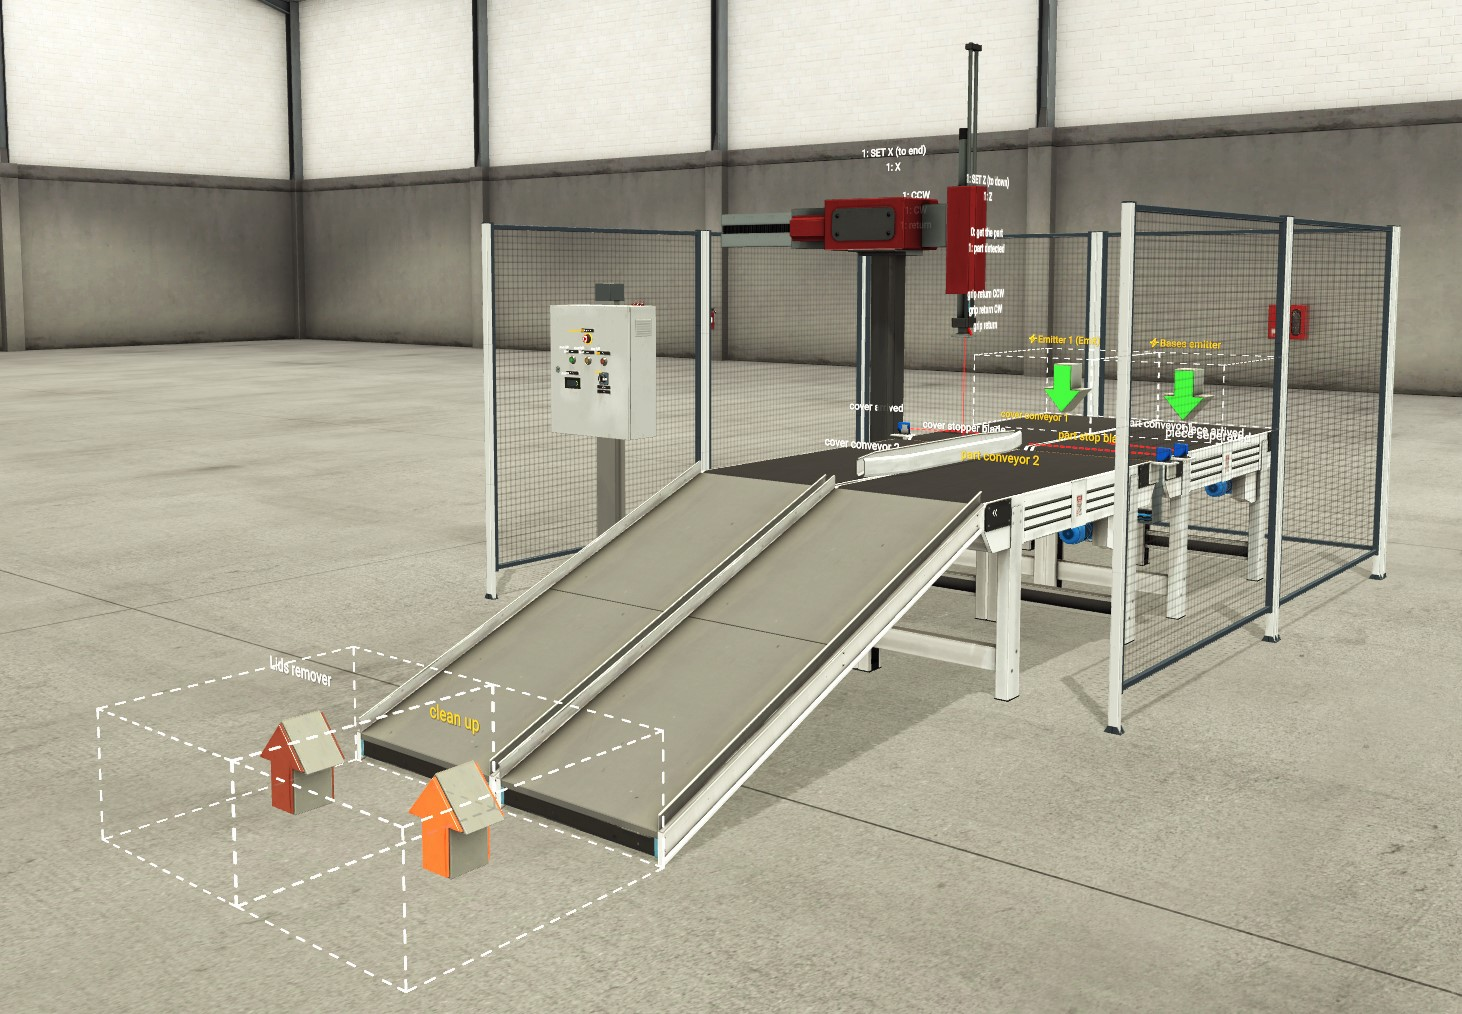
\includegraphics[width=0.5\columnwidth]{imgs/io/1.jpg}
    \caption[Right view of the created system]{Right view of the created system}
    \label{fig-magnitude}
\end{figure}%

The left view of the simulation system is shown in Figure 4.5.
\begin{figure}[H]
    \centering
    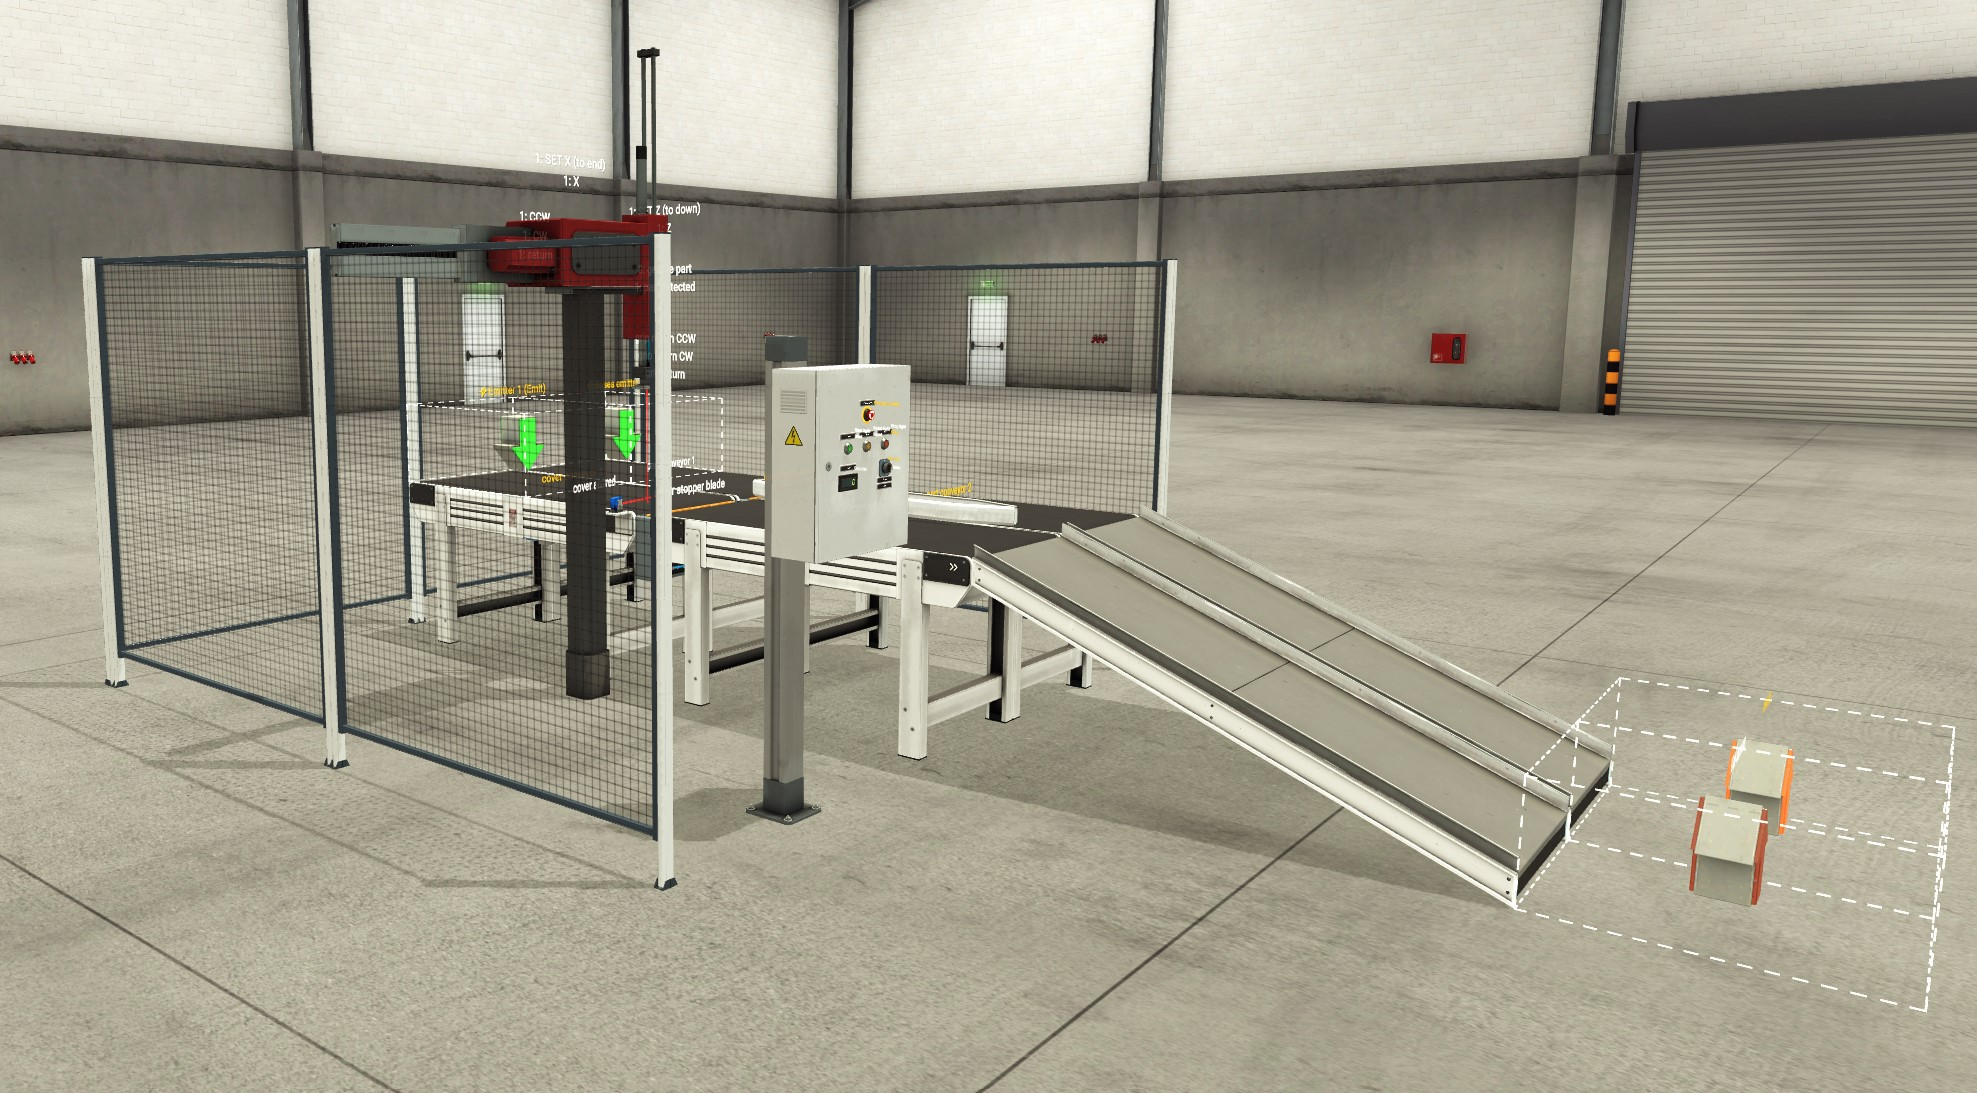
\includegraphics[width=0.5\columnwidth]{imgs/io/2.jpg}
    \caption[Left view of the created system]{Left view of the created system}
    \label{fig-magnitude}
\end{figure}%

\begin{itemize}
    \item \textbf{Working Principle of the System:} 
\end{itemize}

\begin{enumerate}
    \item \textbf{}\textbf{First stage:} When the start button is pressed while the emergency stop button shown in Figure 4.7 is closed, the part and cover conveyor shown in Figure 4.8 will start working.
    \item \textbf{} \textbf{Second stage:} When the created part and the cover are detected by the diffuse sensors seen in blue on both sides, the blades will lift up and the progress of the products on the belt will be stopped.
    \item \textbf{} \textbf{Third stage} The robot arm will come into play and, as seen in Figure 4.9, it will pick up the cover according to the values ​​set for it, place it on the body and drop it.
    \item \textbf{} \textbf{Fourth stage} After the parts are combined, the blade in front of the part will lift and the combined product will continue on the conveyor.
    \item \textbf{} \textbf{Fifth stage:} Finally, the product that has completed its movement on the conveyor will slide down from the platform and be removed as seen in Figure 4.11.
\end{enumerate}

\begin{figure}[H]
    \centering
    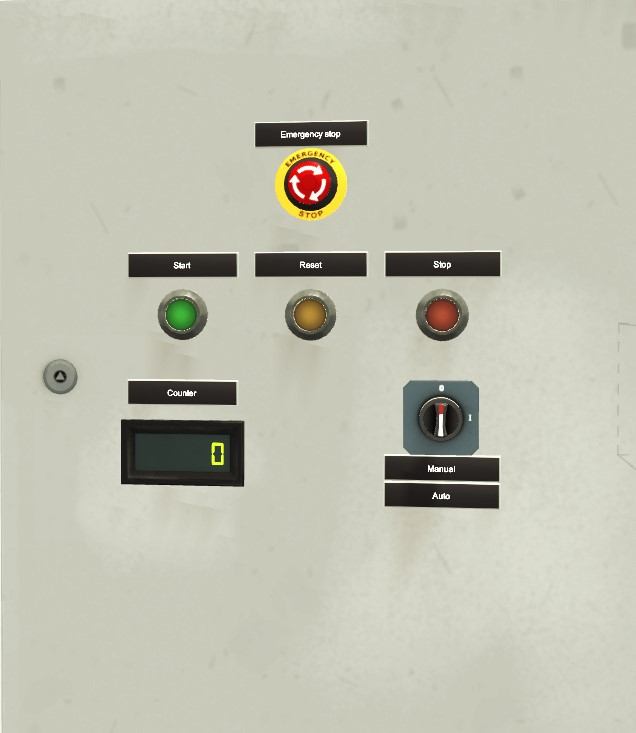
\includegraphics[width=0.65\columnwidth]{imgs/io/5.jpg}
    \caption[Board with buttons]{Board with buttons}
    \label{fig-magnitude}
\end{figure}%
\begin{figure}[H]
    \centering
    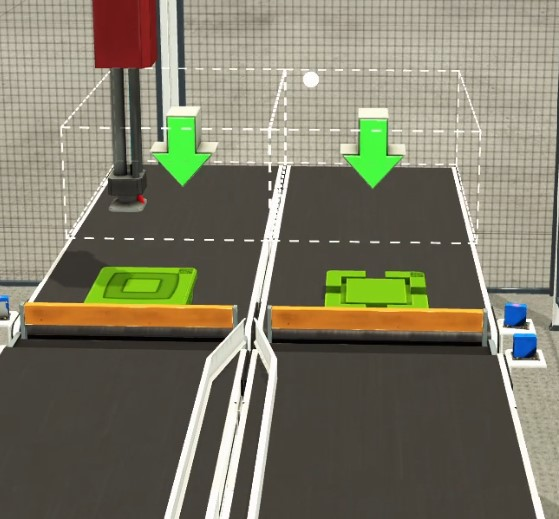
\includegraphics[width=0.65\columnwidth]{imgs/io/9.jpg}
    \caption[Creating parts and covers]{Creating parts and covers}
    \label{fig-magnitude}
\end{figure}%
\begin{figure}[H]
    \centering
    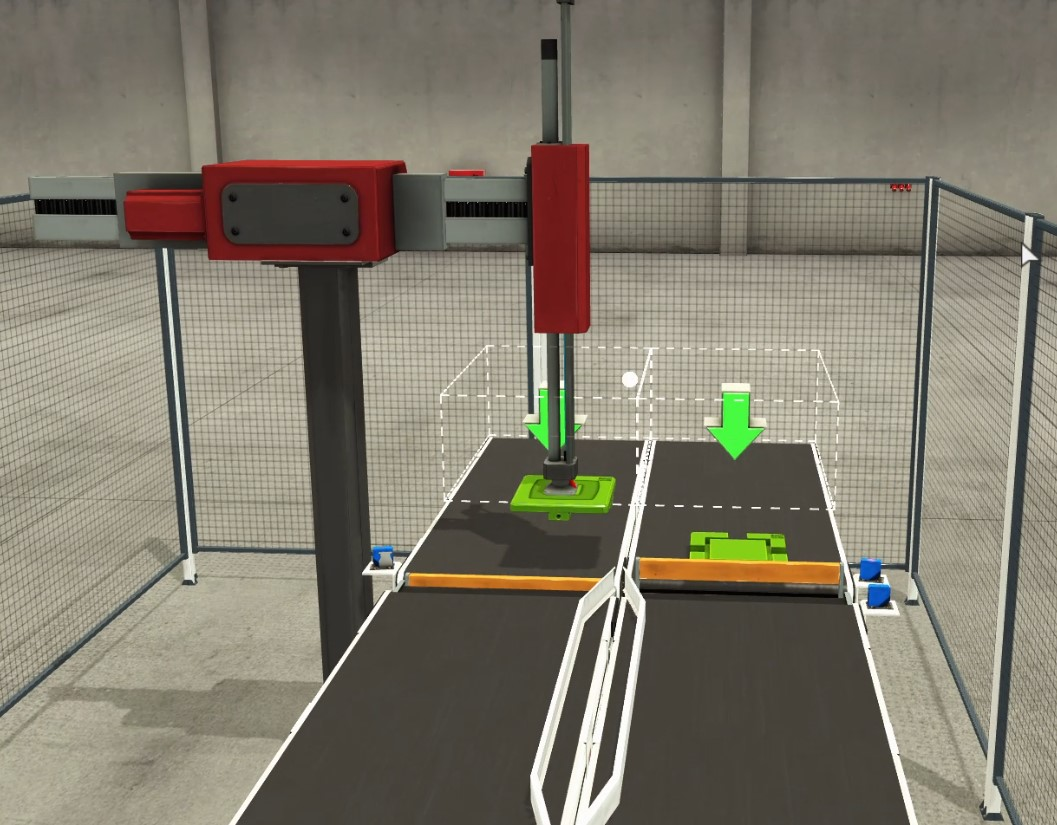
\includegraphics[width=0.8\columnwidth]{imgs/io/8.jpg}
    \caption[Robot arm moves the cover to the body]{Robot arm moves the cover to the body}
    \label{fig-magnitude}
\end{figure}%
\begin{figure}[H]
    \centering
    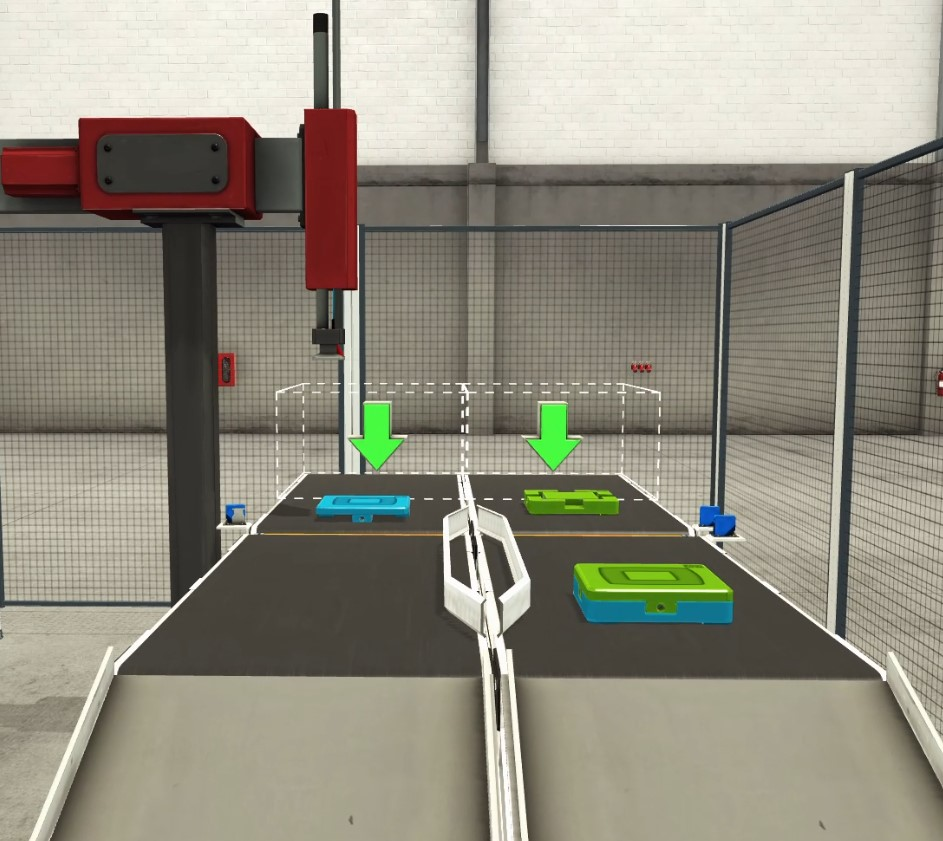
\includegraphics[width=0.8\columnwidth]{imgs/io/7.jpg}
    \caption[After the blades are opened, the produced part moves forward on the conveyor.]{After the blades are opened, the produced part moves forward on the conveyor.}
    \label{fig-magnitude}
\end{figure}%
\begin{figure}[H]
    \centering
    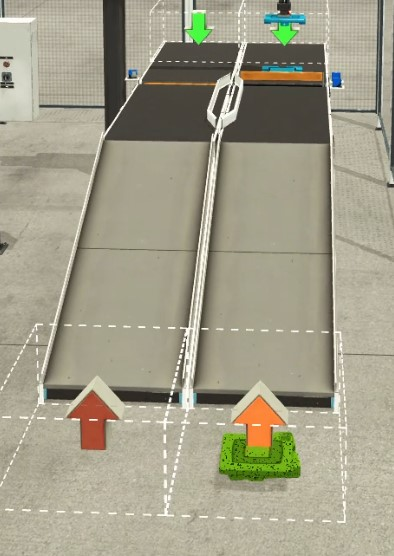
\includegraphics[width=0.5\columnwidth]{imgs/io/10.jpg}
    \caption[The manufactured part completes the conveyor and reaches the final stage.]{The manufactured part completes the conveyor and reaches the final stage.}
    \label{fig-magnitude}
\end{figure}%

All of these processes above are programmed via TIA Portal software and the inputs and outputs are placed in the same positions in the PLC and Factory IO software.
Below is the configuration of inputs and outputs in Factory IO according to PLCSim. The TIA Portal program that enables the operation of the system is presented in detail in Appendix-1.

\begin{figure}[H]
    \centering
    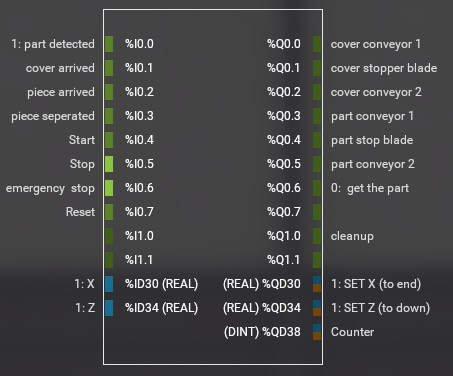
\includegraphics[width=0.5\columnwidth]{imgs/io/11.jpg}
    \caption[S7-1200 PLCSim driver settings]{S7-1200 PLCSim driver settings}
    \label{fig-magnitude}
\end{figure}%

\section{Highlight challenges and how they were addressed}
This project first includes the creation of an industrial production system in the Factory IO environment and the control of this system with a PLC. Then comes the determination and modeling of energy consumption parts. It is aimed to replace the parameters obtained from the industrial system and related to energy consumption in the model and operate with a PID controller at maximum efficiency.

In the part of the project so far, the system has been created, controlled with a PLC, energy consumption elements have been determined and energy-based modeled. The problem encountered is that the energy and parameters of the conveyors and robot arm located in the production facility and causing energy consumption cannot be obtained. The main problem causing this is that the Factory IO program does not have sensors such as an energy analyzer or encoder that will give the rotation speed of the motors directly. In addition, there is no data regarding the type of these motors or the simulation parameters. In other words, only the energy-related parameters of these two components need to be determined in order to complete the project. After this is done, the created model will be replaced and control will be provided with a PID controller. Research on this is ongoing.

Apart from this, while creating the system in Factory IO, a problem was encountered in which the system worked without pressing any buttons, and this was solved with the added emergency stop button. Apart from this, some minor system failures were experienced and easily solved.

In this study, it was aimed to transfer the energy data of the conveyor system to the PLC using the Factory I/O simulation software. However, as a result of the tests, it was not possible to transfer the data related to energy consumption directly to the PLC in the simulation environment at the expected level. Due to these technical limitations experienced during the implementation process, it was decided to evaluate the possibility of continuing with the SCADA (Supervisory Control and Data Acquisition) system, which offers a more stable and measurable structure in the monitoring and control component of the project.

SCADA systems provide high-level visualization, data collection and central control in industrial automation and energy monitoring projects; enabling real-time process monitoring. In this context, parameters such as the operating status of the conveyor system modeled in the Factory I/O environment, the triggering time of the motors, and the active times of the loads in the system can be digitized via the PLC and transferred to the SCADA screen. By using a Ladder diagram to be developed within the PLC, the operating times of the motors can be measured with counters or timers (TON blocks) and the approximate energy consumption can be calculated based on these values. For example, a certain fixed power factor is defined for each motor and the energy consumption data is obtained by multiplying it by the motor operating time. When this data is transferred to the SCADA system, both instantaneous energy consumption and total cumulative consumption can be monitored graphically via the user interface. In addition, thanks to the alarm and reporting features of SCADA; automatic warning systems can be created for situations such as exceeding energy limit values ​​and periodic consumption analyses can be reported. Thus, a realistic and traceable energy management system can be established in the light of the data obtained from the processes created in the simulation environment without using a physical energy analyzer in the field. This approach allows students to develop both PLC programming and SCADA application development competencies in an integrated manner.

\medskip

\clearpage